\namedsection{Ablauf eines Job Scheduling-Prozesses \& Batch Jobs}{T}

Nachdem der Benutzer sich im System über Benutzername/Passwort authentifiziert und einen gültigen JSON Web Token (siehe Kapitel \ref{section:security}) bekommen hat, kann der Benutzer alle verfügbaren Jobs im System sich anzeigen lassen. Dies kann beispielsweise über unser entwickeltes Frontend oder direkt über die bereitgestellten REST APIs der Controller-Klassen geschehen. Wichtig hierbei ist, dass immer ein Mapping der Daten über die Mapper-Beans erfolgt, um ein Leaking des Datenbank-Domänenmodells zu vermeiden. Anschließend kann der Benutzer den gewünschten Job ebenfalls über das Frontend oder über direkt über die REST API starten. Nachdem die Validierungen (z.B. Jobeinstellung vorhanden und gültig) positiv sind, wird der Job asynchron geplant und anschließend in der Datenbank persistiert, um bei Komplikationen beispielsweise einen Neustart des Jobs zu ermöglichen. Abbildung \ref{fig:Ablauf eines Job Scheduling-Prozesses} zeigt den Ablauf für den Prozess eines Job Scheduling-Prozesses.


\begin{figure}[!h]
\centering
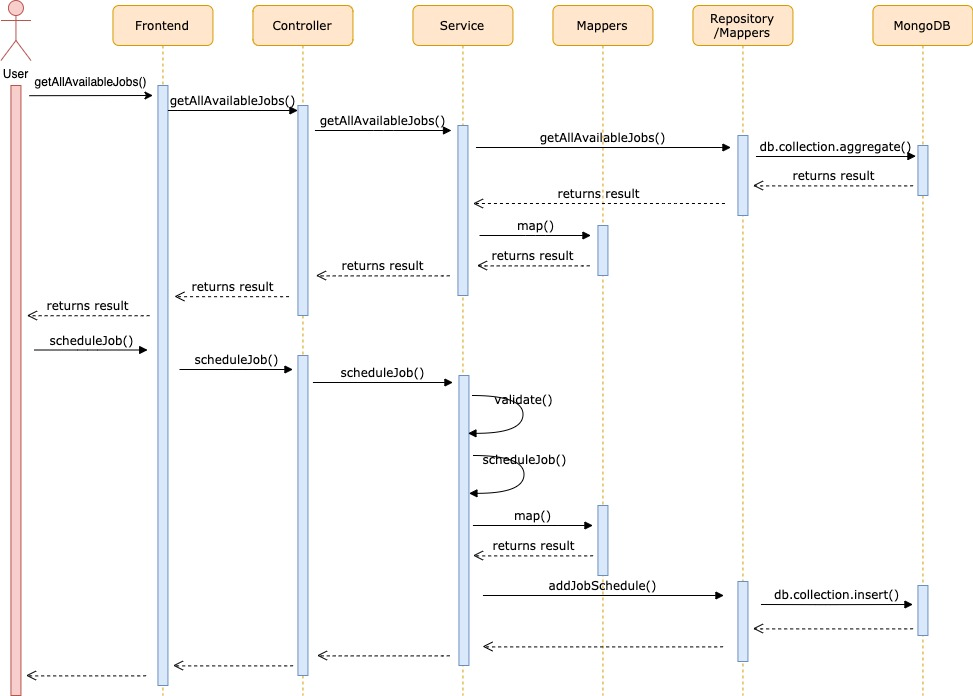
\includegraphics[width=15cm]{images/00_software_architecture/03_job_scheduling_process/scheduling_process.jpg}
\caption{Ablauf eines Job Scheduling-Prozesses}
\label{fig:Ablauf eines Job Scheduling-Prozesses}
\end{figure}

In diesem Kontext wird der Job über eine Spring Bean des Typs QuartzJob ausgelöst, welche eine JobLauncher-Instanz des zu auszuführenden Batch Jobs hält. Dieser Launcher wird dann entsprechend aufgerufen, um den betreffenden Batch Job auszuführen, sobald der Auslösezeitpunkt des Triggers eingetreten ist. Wichtig hierbei ist, dass wir in unserer Implementierung die Daten nach vordefinierten Broken (Chunks) verarbeiten und die Daten schrittweise gelesen, transformiert und gespeichert werden. Demzufolge besteht in unserer Implementierung ein Flow immer aus einem Step, der wiederrum aus einem Leseprozess (MyBatisCursorItemReader), Transformationsprozess (Processor) und einem Schreibprozess (MongoItemWriter) besteht. In diesem Fall werden immer bis zu einer vordefinierten Anzahl an Datensätzen (z.B. 1000) aus der MSSQL-Datenbank gelesen, welche dann in das Ziel-Datenbankmodell transformiert werden, um diese dann anschließend in der MongoDB abzuspeichern. Dieser Prozesse wird dann solange wiederholt bis alle Datensätze aus der MSSQL-Datenbank gelesen und in die MongoDB geschrieben worden sind. Dieser Ansatz hat den Vorteil, dass nur eine begrenzte Datenmenge im Arbeitsspeicher gehalten wird, da die Daten in mehreren Brocken transaktional in die Datenbank geschrieben werden. Nachdem der gesamte Step durchgelaufen ist, wird ein „ExitStatus“ an den Job zurückgegeben, der über den Ausführungserfolg des Jobs berichtet. Die Abbildung \ref{fig:Ablauf eines Batch Jobs} veranschaulicht den Ablauf eines Batch Jobs.

\begin{figure}[!h]
\centering
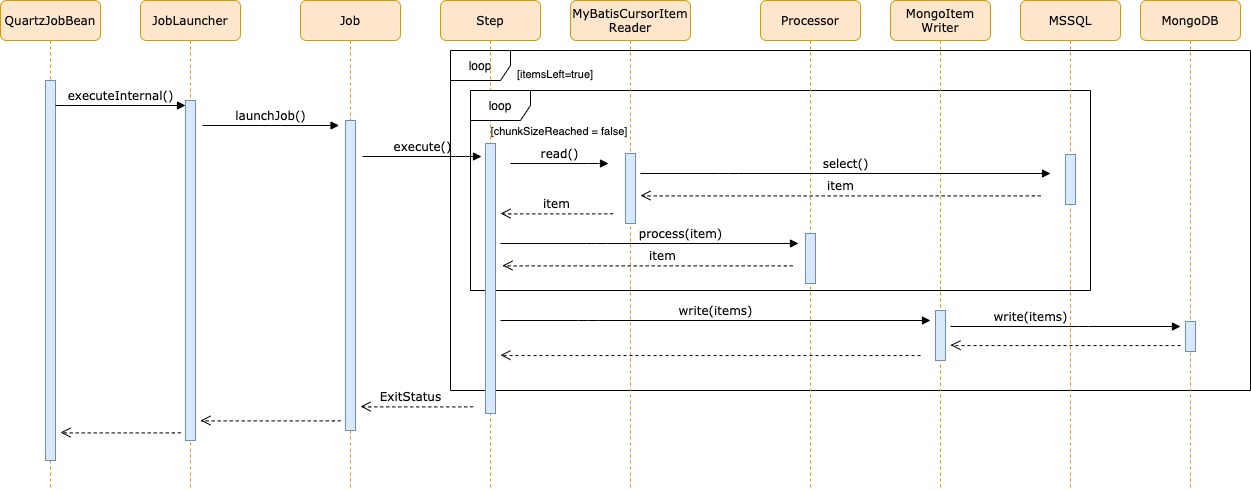
\includegraphics[width=15cm]{images/00_software_architecture/03_job_scheduling_process/job_execution_process.jpg}
\caption{Ablauf eines Batch Jobs}
\label{fig:Ablauf eines Batch Jobs}
\end{figure}